\section{Введение}

Появившись в 2009 году, Real-Time Bidding (RTB) стала важной новой парадигмой в медийной рекламе~\cite{arrival-of-rtb}. Например, по данным IAB/PwC, в США в 2024 году объём RTB оценивается в \$82,2 млрд, что составляет 61\% от всей вычислительной рекламы или 52,8\% от общего объема интернет рекламы~\cite{rtb-growth}. В отличие от прямых продаж рекламных размещений и закупок по заранее согласованным фиксированным ценам, RTB позволяет через аукцион за каждый отдельный показ выбирать наиболее релевантное объявление для конкретного пользователя. Это даёт рекламодателям возможность точнее достигать целевой аудитории и эффективнее расходовать бюджет, а пользователям -- чаще видеть объявления, соответствующие их интересам.

Краткая схема взаимодействия основных компонентов экосистемы RTB показана на Рисунке \ref{fig:rtb-overview}.
\begin{figure}[htbp]
	\centering
	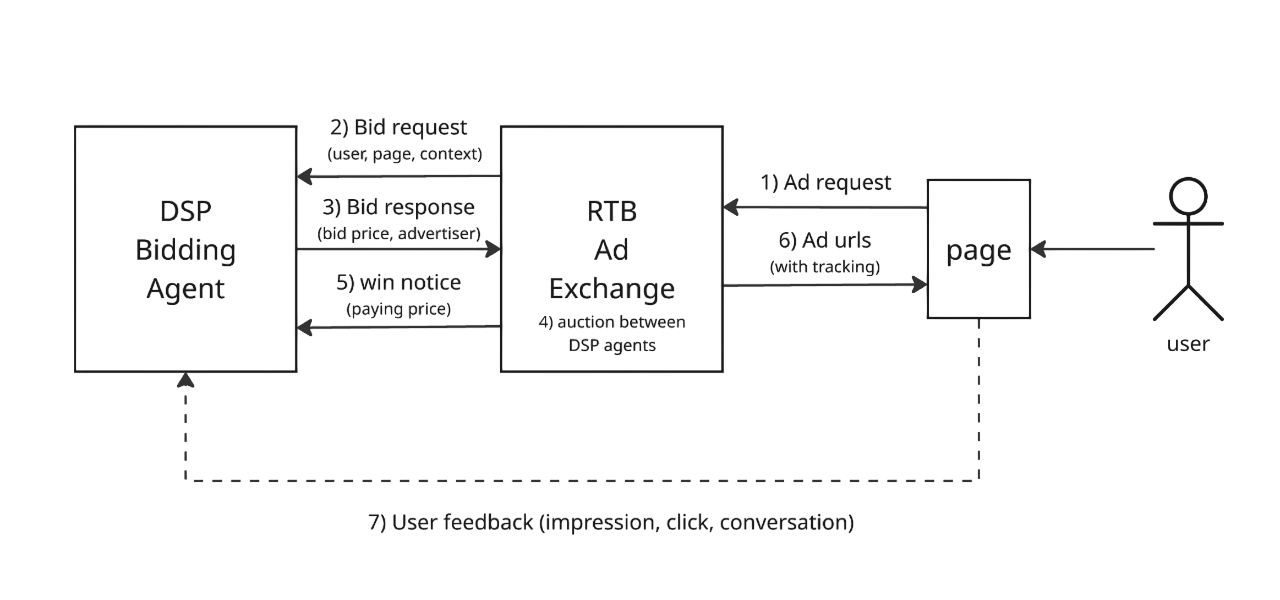
\includegraphics[scale=0.35]{images/rtb_overview.png}
	\caption{Упрощенная иллюстрация взаимодействия между пользователем, рекламной биржей и DSP}
	\label{fig:rtb-overview}
\end{figure}
Процесс начинается с того, что пользователь посещает сайт/приложение, содержащее рекламный инвентарь: при загрузке страницы клиент отправляет запрос в рекламную биржу (ad exchange), чтобы определить, какое рекламное объявление будет показано в доступном рекламном слоте и по какой цене (этап 1 на Рис.~\ref{fig:rtb-overview}).

Далее биржа рассылает запросы на ставки (bid requests) в различные автоматизированные системы покупки рекламы (Demand-Side Platforms, DSP) (этап 2 на Рис.~\ref{fig:rtb-overview}). Запрос ставки обычно содержит сведения об издателе и контексте размещения (например, URL/домен, тематика, характеристики рекламного слота), а также признаки пользователя (чаще всего идентификаторы на основе cookie/устройств) и технические параметры (тип устройства, ОС, браузер и т.п.).

Получив запрос, DSP решает две ключевые задачи:
\begin{enumerate}
  \item[(1)] Следует ли участвовать в аукционе и от имени какого рекламодателя/кампании
  (в зависимости от таргетинга, ограничений бюджета и частотных ограничений);
  \item[(2)] Eсли участвовать, то вычислить величину ставки.
\end{enumerate}
После этого DSP отправляет свой ответ (bid response) обратно на биржу (этап 3 на Рис.~\ref{fig:rtb-overview}).

Рекламная биржа проводит аукцион после получения ответов от всех DSP либо по истечении лимита по времени (этап 4 на Рис.~\ref{fig:rtb-overview}). На практике часто используется аукцион Викри, также известный как аукцион второй цены: участник с наибольшей ставкой выигрывает показ, но платит цену, близкую ко второй по величине ставке. После определения победителя биржа уведомляет выигравшую DSP о факте победы и цене (win notice) (этап 5 на Рис.~\ref{fig:rtb-overview}).

Далее биржа возвращает на страницу параметры показа/ссылки на креатив (этап 6 на Рис.~\ref{fig:rtb-overview}); клиент загружает креатив с рекламного сервера, и пользователь видит объявление на площадке издателя. Если объявление заинтересовало пользователя, он может кликнуть по нему и перейти на страницу рекламодателя, а затем совершить целевое действие (conversion). Эти события (показ, клик, конверсия) формируют пользовательскую обратную связь, которая через механизмы трекинга передаётся участникам цепочки и используется для оптимизации закупки (этап 7 на Рис.~\ref{fig:rtb-overview}).

Хорошо известно, что длительная загрузка страницы значительно снижает удовлетворённость пользователей~\cite{need-web-speed}, поэтому DSP обычно обязаны возвращать ставку в очень короткие сроки (например, 100 мс).
Более подробные сведения об RTB можно найти в статьях~\cite{arrival-of-rtb, rtb-research}.

Цель оптимизации алгоритма назначения ставок на стороне DSP -- улучшение ключевых показателей эффективности (Key Performance Indicator -- KPI) рекламодателей, таких как число кликов и/или число конверсий при фиксированном бюджете кампании. Поэтому алгоритм назначения ставок является ключевым компонентом успешной DSP: именно здесь вычислительная реклама напрямую опирается на анализ больших данных (Big Data) и аналитическую инфраструктуру (сбор событий, мониторинг качества трафика, контроль бюджетов и ограничений). Проектирование алгоритма ставок затрагивает множество областей компьютерных наук, включая машинное обучение, анализ данных, статистику, оптимизацию и теорию игр.

Несмотря на популярность, исследователям из академической среды почти невозможно получить доступ к чувствительным и потому строго защищённым данным. К счастью, в 2013 году iPinYou провела международное соревнование по алгоритмам RTB, состоявшее из трёх сезонов, основная задача которого была -- решение проблемы оптимизации ставок DSP (DSP Bid Optimisation Problem). В марте 2014 года набор данных, использованный в трёх сезонах соревнования, был опубликован для исследовательских целей~\cite{ipinyou-contest-database}. Насколько известно, это первый крупный набор данных RTB в публичном доступе. 

Для работы с данным объёмом и структурой логов целесообразно использовать систему управления базами данных (СУБД): это упрощает повторяемые аналитические запросы, обеспечивает воспроизводимость расчётов, централизует хранение и контроль качества данных, а также позволяет эффективно агрегировать события на больших выборках. В рамках работы используется ClickHouse -- колоночная СУБД, ориентированная на высокопроизводительную аналитическую обработку. ClickHouse хорошо подходит для задач статистического анализа логов RTB благодаря эффективному сжатию колонок, быстрому выполнению агрегирующих запросов по большим таблицам, поддержке материализованных представлений/вычисляемых столбцов и возможности масштабирования под рост объёма данных. Например, по сравнению с другой популярной СУБД PostgreSQL -- ClickHouse в типовых аналитических запросах может обеспечивать более чем 20-кратное ускорение выполнения~\cite{clickhouse-vs-postgres}.

Для интерактивной визуализации результатов анализа и подготовки воспроизводимых отчётов в работе используется Yandex DataLens -- BI-инструмент для построения дашбордов и исследовательской аналитики. DataLens позволяет подключаться к ClickHouse как к источнику данных, создавать графики и таблицы поверх SQL-запросов, применять фильтры и сегментацию (например, по кампаниям, доменам, типам устройств и времени), а также публиковать единый набор визуализаций для последующей проверки и интерпретации результатов, обновляемый в реальном времени. Использование BI-слоя снижает необходимость ручной генерации графиков в коде, ускоряет итерации анализа и упрощает сравнение метрик в различных разрезах.

В этой работе мы сначала проведём описательный обзор набора данных и его основных сущностей, затем выполним подготовку данных: предобработку с использованием Python, валидацию структуры и типов для последующей загрузки в ClickHouse, а также материализацию отдельных вычисляемых столбцов в базе данных для оптимизации типовых запросов. Далее будет выполнен детальный анализ RTB-аукционов и рассчитаны ключевые метрики эффективности рекламных кампаний: Cost Per Mille (CPM), Click-Through Rate (CTR), Conversion Rate (CVR), Effective Cost Per Click (eCPC), Effective Cost Per Action (eCPA). Отдельное внимание будет уделено влиянию факторов контекста и пользователя на указанные метрики, включая тип устройства, браузер, время (час/день недели), характеристики рекламного слота. Наконец, будет построена RTB-воронка и подготовлены визуализации с использованием DataLens.

\subsection{Цель}
Цель работы заключается в выявлении наиболее значимых показателей эффективности путем анализа и визуализации результатов RTB-аукционов на примере открытого набора данных iPinYou с помощью DataLens для решения бизнес задач.

\subsection{Объект исследования}
Объектом исследования являются данные RTB-аукционов iPinYou, опубликованные для исследовательских целей по итогам соревнования iPinYou RTB Bidding Algorithm Competition.

\subsection{Предмет исследования}
Предметом исследования являются закономерности и статистические зависимости в данных RTB-аукционов, определяющие результаты рекламного показа и эффективность кампаний: влияние параметров рекламного слота и площадки, времени, устройства и доступных пользовательских признаков на вероятность клика/конверсии, а также на стоимость закупки инвентаря в рамках ограничений бюджета.

\subsection{Методы исследования}
\begin{itemize}
    \item Предобработка и анализ данных с использованием Python (очистка, валидация, преобразование признаков).
    \item Хранение и аналитическая обработка данных в колоночной СУБД ClickHouse (SQL-запросы, агрегирование таблиц, материализация вычисляемых столбцов).
    \item Построение воронки событий и расчёт рекламных метрик (CPM, CTR, CVR, eCPC, eCPA) в различных срезах и сегментах с использованием Yandex DataLens.
    \item Анализ и визуализация чартов с использованием Yandex DataLens. Построение интерактивного дашборда.
    \item Обзор академических и прикладных источников по RTB и оптимизации ставок~\cite{rtb-research, rtb-benchmarking}.
\end{itemize}

\subsection{Задачи}
Задачи проекта разделяются на две части: исследовательскую и программную.

\begin{itemize}
  \item \textbf{Исследовательская часть}
    \begin{itemize}
        \item Провести описательный обзор набора данных iPinYou и основных сущностей логов (bidding log / impression log / click log / conversion log).
        \item Выполнить расчёт и интерпретацию ключевых показателей рекламных кампаний: CPM, CTR, CVR, eCPC, eCPA.
        \item Построить RTB-воронку и оценить потери на каждом этапе.
        \item Проанализировать влияние факторов контекста и пользователя на метрики эффективности (тип устройства, время, параметры площадки и слота, доступные признаки пользовательского сегмента).
        \item Пройти курс «DataLens: анализ и визуализация данных» для освоения инструментария построения дашбордов.
    \end{itemize}

  \item \textbf{Программная часть}
      \begin{itemize}
        \item Подготовить пайплайн предобработки данных в Python: очистка, нормализация форматов.
        \item Развернуть в облаке базу данных и загрузить подготовленные таблицы.
        \item Реализовать оптимизации для повторяющегося анализа (агрегации, вычисляемые столбцы/материализованные представления).
        \item Провести расчет метрик и подготовить визуализации в различных разрезах.
        \item Построить дашборды в Yandex DataLens для интерактивного анализа метрик и сравнения сегментов.
      \end{itemize}
\end{itemize}

\subsection{Актуальность работы}
Актуальность работы обусловлена тем, что RTB является доминирующим механизмом закупки медийной рекламы и формирует значительную часть рынка интернет-рекламы. Набор данных iPinYou предоставляет редкую возможность исследовать реальные логи аукционов и проверить статистические гипотезы о факторах эффективности кампаний. Дополнительно, использование связки ClickHouse + DataLens позволяет выстроить воспроизводимый контур хранения, расчёта и визуализации метрик, применимый к анализу рекламных логов большого объёма в практических бизнес задачах. Таким образом, можно считать, что актуальность работы продемонстрирована.


\subsection{План работы}

План выполнения работ и сроки по этапам приведены в Таблице~\ref{tab:work_plan}.
Графическое представление плана (диаграмма Ганта) показано на Рис.~\ref{fig:gantt}.

\begin{table}[h!]
  \begin{center}
    \caption{Календарный план выполнения работы}
    \label{tab:work_plan}
    \renewcommand{\arraystretch}{1.15}
    \begin{tabular}{c|p{6.8cm}|c|c}
      \textbf{N} & \textbf{Задача} & \textbf{Дата начала} & \textbf{Дата окончания} \\
      \hline
      1  & Обзор литературы по RTB & 02.11.2025 & 30.11.2025 \\
      2  & Освоение Yandex DataLens & 02.11.2025 & 11.01.2026 \\
      3  & Обзор датасета iPinYou & 15.11.2025 & 29.11.2025 \\
      4  & Предобработка данных & 04.12.2025 & 21.12.2025 \\
      5  & Развёртывание БД и загрузка таблиц & 10.12.2025 & 11.01.2026 \\
      6  & Оптимизация аналитических запросов & 05.01.2026 & 16.01.2026 \\
      7  & Расчёт ключевых метрик эффективности & 16.01.2026 & 31.01.2026 \\
      8  & Построение RTB-воронки и потерь & 20.01.2026 & 28.02.2026 \\
      9  & Факторный анализ эффективности & 01.02.2026 & 14.03.2026 \\
      10 & Визуализации и анализ метрик по срезам & 14.03.2026 & 10.04.2026 \\
      11 & Построение дашбордов в DataLens & 01.02.2026 & 20.04.2026 \\
      12 & Сопоставление с литературой и выводы & 20.04.2026 & 25.04.2026 \\
    \end{tabular}
  \end{center}
\end{table}


\begin{figure}[htbp]
    \centering
    \caption{Диаграмма Ганта плана выполнения работы}

    \label{fig:gantt}
    \begin{ganttchart}[
        time slot format=isodate,
        x unit=0.085cm,
        y unit chart=1.3cm,
        y unit title=1.0cm,
        bar height=0.55,
        hgrid,
        inline,
        title/.style={draw=black, fill=white},
        title label font=\small\bfseries,
        bar/.style={draw=black, fill=gray!55},
        bar label font=\small\bfseries,
        bar label node/.append style={align=center}
    ]{2025-11-02}{2026-04-30}
      \gantttitlecalendar{year, month=shortname} \\
      \ganttbar{1}{2025-11-02}{2025-11-30} \\
      \ganttbar{2}{2025-11-02}{2026-01-11} \\
      \ganttbar{3}{2025-11-15}{2025-11-29} \\
      \ganttbar{4}{2025-12-04}{2025-12-21} \\
      \ganttbar{5}{2025-12-10}{2026-01-11} \\
      \ganttbar{6}{2026-01-05}{2026-01-16} \\
      \ganttbar{7}{2026-01-16}{2026-01-31} \\
      \ganttbar{8}{2026-01-20}{2026-02-28} \\
      \ganttbar{9}{2026-02-01}{2026-03-14} \\
      \ganttbar{10}{2026-03-14}{2026-04-10} \\
      \ganttbar{11}{2026-02-01}{2026-04-20} \\
      \ganttbar{12}{2026-04-20}{2026-04-25}
    \end{ganttchart}
\end{figure}
